% Options for packages loaded elsewhere
\PassOptionsToPackage{unicode}{hyperref}
\PassOptionsToPackage{hyphens}{url}
\PassOptionsToPackage{dvipsnames,svgnames,x11names}{xcolor}
%
\documentclass[
  letterpaper,
  DIV=11,
  numbers=noendperiod]{scrartcl}

\usepackage{amsmath,amssymb}
\usepackage{iftex}
\ifPDFTeX
  \usepackage[T1]{fontenc}
  \usepackage[utf8]{inputenc}
  \usepackage{textcomp} % provide euro and other symbols
\else % if luatex or xetex
  \usepackage{unicode-math}
  \defaultfontfeatures{Scale=MatchLowercase}
  \defaultfontfeatures[\rmfamily]{Ligatures=TeX,Scale=1}
\fi
\usepackage{lmodern}
\ifPDFTeX\else  
    % xetex/luatex font selection
\fi
% Use upquote if available, for straight quotes in verbatim environments
\IfFileExists{upquote.sty}{\usepackage{upquote}}{}
\IfFileExists{microtype.sty}{% use microtype if available
  \usepackage[]{microtype}
  \UseMicrotypeSet[protrusion]{basicmath} % disable protrusion for tt fonts
}{}
\makeatletter
\@ifundefined{KOMAClassName}{% if non-KOMA class
  \IfFileExists{parskip.sty}{%
    \usepackage{parskip}
  }{% else
    \setlength{\parindent}{0pt}
    \setlength{\parskip}{6pt plus 2pt minus 1pt}}
}{% if KOMA class
  \KOMAoptions{parskip=half}}
\makeatother
\usepackage{xcolor}
\setlength{\emergencystretch}{3em} % prevent overfull lines
\setcounter{secnumdepth}{-\maxdimen} % remove section numbering
% Make \paragraph and \subparagraph free-standing
\ifx\paragraph\undefined\else
  \let\oldparagraph\paragraph
  \renewcommand{\paragraph}[1]{\oldparagraph{#1}\mbox{}}
\fi
\ifx\subparagraph\undefined\else
  \let\oldsubparagraph\subparagraph
  \renewcommand{\subparagraph}[1]{\oldsubparagraph{#1}\mbox{}}
\fi


\providecommand{\tightlist}{%
  \setlength{\itemsep}{0pt}\setlength{\parskip}{0pt}}\usepackage{longtable,booktabs,array}
\usepackage{calc} % for calculating minipage widths
% Correct order of tables after \paragraph or \subparagraph
\usepackage{etoolbox}
\makeatletter
\patchcmd\longtable{\par}{\if@noskipsec\mbox{}\fi\par}{}{}
\makeatother
% Allow footnotes in longtable head/foot
\IfFileExists{footnotehyper.sty}{\usepackage{footnotehyper}}{\usepackage{footnote}}
\makesavenoteenv{longtable}
\usepackage{graphicx}
\makeatletter
\def\maxwidth{\ifdim\Gin@nat@width>\linewidth\linewidth\else\Gin@nat@width\fi}
\def\maxheight{\ifdim\Gin@nat@height>\textheight\textheight\else\Gin@nat@height\fi}
\makeatother
% Scale images if necessary, so that they will not overflow the page
% margins by default, and it is still possible to overwrite the defaults
% using explicit options in \includegraphics[width, height, ...]{}
\setkeys{Gin}{width=\maxwidth,height=\maxheight,keepaspectratio}
% Set default figure placement to htbp
\makeatletter
\def\fps@figure{htbp}
\makeatother
% definitions for citeproc citations
\NewDocumentCommand\citeproctext{}{}
\NewDocumentCommand\citeproc{mm}{%
  \begingroup\def\citeproctext{#2}\cite{#1}\endgroup}
\makeatletter
 % allow citations to break across lines
 \let\@cite@ofmt\@firstofone
 % avoid brackets around text for \cite:
 \def\@biblabel#1{}
 \def\@cite#1#2{{#1\if@tempswa , #2\fi}}
\makeatother
\newlength{\cslhangindent}
\setlength{\cslhangindent}{1.5em}
\newlength{\csllabelwidth}
\setlength{\csllabelwidth}{3em}
\newenvironment{CSLReferences}[2] % #1 hanging-indent, #2 entry-spacing
 {\begin{list}{}{%
  \setlength{\itemindent}{0pt}
  \setlength{\leftmargin}{0pt}
  \setlength{\parsep}{0pt}
  % turn on hanging indent if param 1 is 1
  \ifodd #1
   \setlength{\leftmargin}{\cslhangindent}
   \setlength{\itemindent}{-1\cslhangindent}
  \fi
  % set entry spacing
  \setlength{\itemsep}{#2\baselineskip}}}
 {\end{list}}
\usepackage{calc}
\newcommand{\CSLBlock}[1]{\hfill\break\parbox[t]{\linewidth}{\strut\ignorespaces#1\strut}}
\newcommand{\CSLLeftMargin}[1]{\parbox[t]{\csllabelwidth}{\strut#1\strut}}
\newcommand{\CSLRightInline}[1]{\parbox[t]{\linewidth - \csllabelwidth}{\strut#1\strut}}
\newcommand{\CSLIndent}[1]{\hspace{\cslhangindent}#1}

\KOMAoption{captions}{tableheading}
\makeatletter
\@ifpackageloaded{caption}{}{\usepackage{caption}}
\AtBeginDocument{%
\ifdefined\contentsname
  \renewcommand*\contentsname{Table of contents}
\else
  \newcommand\contentsname{Table of contents}
\fi
\ifdefined\listfigurename
  \renewcommand*\listfigurename{List of Figures}
\else
  \newcommand\listfigurename{List of Figures}
\fi
\ifdefined\listtablename
  \renewcommand*\listtablename{List of Tables}
\else
  \newcommand\listtablename{List of Tables}
\fi
\ifdefined\figurename
  \renewcommand*\figurename{Figure}
\else
  \newcommand\figurename{Figure}
\fi
\ifdefined\tablename
  \renewcommand*\tablename{Table}
\else
  \newcommand\tablename{Table}
\fi
}
\@ifpackageloaded{float}{}{\usepackage{float}}
\floatstyle{ruled}
\@ifundefined{c@chapter}{\newfloat{codelisting}{h}{lop}}{\newfloat{codelisting}{h}{lop}[chapter]}
\floatname{codelisting}{Listing}
\newcommand*\listoflistings{\listof{codelisting}{List of Listings}}
\makeatother
\makeatletter
\makeatother
\makeatletter
\@ifpackageloaded{caption}{}{\usepackage{caption}}
\@ifpackageloaded{subcaption}{}{\usepackage{subcaption}}
\makeatother
\ifLuaTeX
  \usepackage{selnolig}  % disable illegal ligatures
\fi
\usepackage{bookmark}

\IfFileExists{xurl.sty}{\usepackage{xurl}}{} % add URL line breaks if available
\urlstyle{same} % disable monospaced font for URLs
\hypersetup{
  pdftitle={Analyzing Satellite Scaling Bias Using Drone Data, Application to Microphytobenthos Studies},
  colorlinks=true,
  linkcolor={blue},
  filecolor={Maroon},
  citecolor={Blue},
  urlcolor={Blue},
  pdfcreator={LaTeX via pandoc}}

\title{Analyzing Satellite Scaling Bias Using Drone Data, Application to
Microphytobenthos Studies}
\author{Augustin Debly}
\date{}

\begin{document}
\maketitle

\section{Introduction}\label{introduction}

\subsection{MPB}\label{mpb}

The present study focuses on microphytobenthos (MPB) colonizing
estuarine intertidal zones. MPB refers to photosynthetic unicellular
microalgae forming biofilms at the sediment surface during low tides.
This group includes diatoms, euglenids, cyanobacteria, and chlorophyta
(Underwood 2001). They can be associated to mud and sand, i.e.~inorganic
particles with size between 4 and 63µm, and 63 and 2000µm, respectively
(Wentworth 1922). In these soft-bottom sediments, MPB can be the main
primary producer, notably in turbid estuaries.

\subsection{Ecological services}\label{ecological-services}

MPB provides several ecosystem services (Hope, Paterson, and Thrush
2020). In addition to its contribution to carbon fluxes, estimated
between 30 and 230 g C/m²/year (Heip et al. 1995; Park et al. 2024), it
stabilizes the sediment through the secretion of extracellular polymeric
substances (EPS) (Gibbs 1983; Riethmüller et al. 2000; Stal 2010;
Huiming, Hongwei, and Minghong 2011; Fang et al. 2012; Gerbersdorf et
al. 2020), and therefore reduces coastal erosion (Hope, Paterson, and
Thrush 2020). It is a key element of food webs (Deppe 1999;
Aberle-Malzahn 2004; Dauvin and Desroy 2005), and it plays an important
role in nutrient cycling, increasing water quality. It can also be used
as a bioindicator of water quality (Oiry and Barillé 2021).

\subsection{Spatial structure}\label{spatial-structure}

The MPB exhibits spatial variability at different scales

\phantomsection\label{cell-fig-resolutions}
\begin{figure}[H]

\centering{

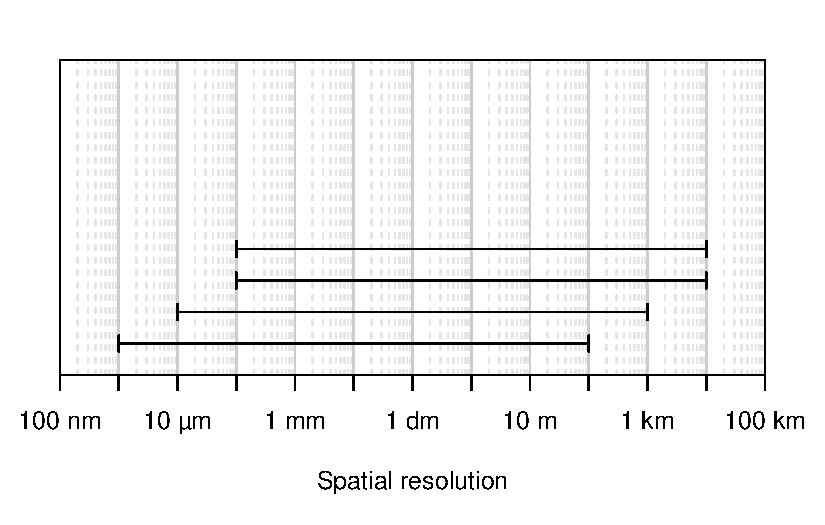
\includegraphics{index_files/figure-pdf/fig-resolutions-1.pdf}

}

\caption{\label{fig-resolutions}Resolutions of x different sensors cross
represented with the different spatial scales of MPB}

\end{figure}%

\textsubscript{Source:
\href{https://AugustinDebly.github.io/Scaling_bias/index.qmd.html}{Article
Notebook}}

\subsection{MPB \& RS}\label{mpb-rs}

\subsection{The use of a proxy}\label{the-use-of-a-proxy}

NDVI can be transformed into biomass following Equation~\ref{eq-NDVIB}

\begin{equation}\phantomsection\label{eq-NDVIB}{
B_{a,b,c}(NDVI) = \frac{1}{c}ln\left(\frac{b}{a+b-NDVI}\right)
}\end{equation}

\subsection{Bias}\label{bias}

\subsection{Present study}\label{present-study}

\section{Material and methods}\label{material-and-methods}

\subsection{Simulating a satellite dataset from a drone
dataset}\label{simulating-a-satellite-dataset-from-a-drone-dataset}

The choice has been made to simulate coarser dataset from drone
fine-scale

\subsection{}\label{section}

\section{Results}\label{results}

\section{Discussion}\label{discussion}

\section*{References}\label{references}
\addcontentsline{toc}{section}{References}

\phantomsection\label{refs}
\begin{CSLReferences}{1}{0}
\bibitem[\citeproctext]{ref-aberle-malzahn_microphytobenthos_2004}
Aberle-Malzahn, Nicole. 2004. {``The Microphytobenthos and Its Role in
Aquatic Food Webs.''} PhD thesis, Christian-Albrechts-Universität Kiel.
\url{https://pure.mpg.de/pubman/faces/ViewItemOverviewPage.jsp?itemId=item_1507232}.

\bibitem[\citeproctext]{ref-dauvin_food_2005}
Dauvin, Jean-Claude, and Nicolas Desroy. 2005. {``The Food Web in the
Lower Part of the {Seine} Estuary: A Synthesis of Existing Knowledge.''}
\emph{Hydrobiologia} 540 (1): 13--27.
\url{https://doi.org/10.1007/s10750-004-7101-3}.

\bibitem[\citeproctext]{ref-deppe_intertidal_1999}
Deppe, Frauke. 1999. {``Intertidal {Mudflats} {Worldwide}.''}

\bibitem[\citeproctext]{ref-fang_effect_2012}
Fang, Hongwei, Huiming Zhao, Qianqian Shang, and Minghong Chen. 2012.
{``Effect of Biofilm on the Rheological Properties of Cohesive
Sediment.''} \emph{Hydrobiologia} 694 (1): 171--81.
\url{https://doi.org/10.1007/s10750-012-1140-y}.

\bibitem[\citeproctext]{ref-gerbersdorf_exploring_2020}
Gerbersdorf, Sabine Ulrike, Kaan Koca, Dirk de Beer, Arjun Chennu,
Christian Noss, Ute Risse-Buhl, Markus Weitere, et al. 2020.
{``Exploring Flow-Biofilm-Sediment Interactions: {Assessment} of Current
Status and Future Challenges.''} \emph{Water Research} 185 (October):
116182. \url{https://doi.org/10.1016/j.watres.2020.116182}.

\bibitem[\citeproctext]{ref-gibbs_effect_1983}
Gibbs, Ronald J. 1983. {``Effect of Natural Organic Coatings on the
Coagulation of Particles.''} \emph{Environmental Science \& Technology}
17 (4): 237--40. \url{https://doi.org/10.1021/es00110a011}.

\bibitem[\citeproctext]{ref-heip_production_1995}
Heip, C. H. R., N. K. Goosen, P. M. J. Herman, J. Kromkamp, J. J.
Middelburg, and K. Soetaert. 1995. {``Production and Consumption of
Biological Particles in Temperate Tidal Estuaries.''} \emph{Oceanography
and Marine Biology: An Annual Review}.
\url{https://www.lifewatch.be/en/imis?module=ref&refid=8311&printversion=1&dropIMIStitle=1}.

\bibitem[\citeproctext]{ref-hope_role_2020}
Hope, Julie A., David M. Paterson, and Simon F. Thrush. 2020. {``The
Role of Microphytobenthos in Soft-Sediment Ecological Networks and Their
Contribution to the Delivery of Multiple Ecosystem Services.''}
\emph{Journal of Ecology} 108 (3): 815--30.
\url{https://doi.org/10.1111/1365-2745.13322}.

\bibitem[\citeproctext]{ref-huiming_floc_2011}
Huiming, Zhao, Fang Hongwei, and Chen Minghong. 2011. {``Floc
Architecture of Bioflocculation Sediment by {ESEM} and {CLSM}.''}
\emph{Scanning} 33 (6): 437--45.
\url{https://doi.org/10.1002/sca.20247}.

\bibitem[\citeproctext]{ref-oiry_using_2021}
Oiry, Simon, and Laurent Barillé. 2021. {``Using Sentinel-2 Satellite
Imagery to Develop Microphytobenthos-Based Water Quality Indices in
Estuaries.''} \emph{Ecological Indicators} 121 (February): 107184.
\url{https://doi.org/10.1016/j.ecolind.2020.107184}.

\bibitem[\citeproctext]{ref-park_harnessing_2024}
Park, Jihae, Hojun Lee, Jana Asselman, Colin Janssen, Stephen Depuydt,
Jonas De Saeger, Thomas Friedl, et al. 2024. {``Harnessing the Power of
Tidal Flat Diatoms to Combat Climate Change.''} \emph{Critical Reviews
in Environmental Science and Technology} 0 (0): 1--22.
\url{https://doi.org/10.1080/10643389.2024.2315004}.

\bibitem[\citeproctext]{ref-riethmuller_chlorophyll_2000}
Riethmüller, R., M. Heineke, H. Kühl, and R. Keuker-Rüdiger. 2000.
{``Chlorophyll a Concentration as an Index of Sediment Surface
Stabilisation by Microphytobenthos?''} \emph{Continental Shelf Research}
20 (10-11): 1351--72.
\url{https://doi.org/10.1016/S0278-4343(00)00027-3}.

\bibitem[\citeproctext]{ref-stal_microphytobenthos_2010}
Stal, Lucas J. 2010. {``Microphytobenthos as a Biogeomorphological Force
in Intertidal Sediment Stabilization.''} \emph{Ecological Engineering},
Special {Issue}: {BioGeoCivil} {Engineering}, 36 (2): 236--45.
\url{https://doi.org/10.1016/j.ecoleng.2008.12.032}.

\bibitem[\citeproctext]{ref-underwood_microphytobenthos_2001}
Underwood, G. J. C. 2001. {``Microphytobenthos.''} In \emph{Encyclopedia
of {Ocean} {Sciences}}, edited by John H. Steele, 1770--77. Oxford:
Academic Press. \url{https://doi.org/10.1006/rwos.2001.0213}.

\bibitem[\citeproctext]{ref-wentworth_scale_1922}
Wentworth, Chester K. 1922. {``A {Scale} of {Grade} and {Class} {Terms}
for {Clastic} {Sediments}.''} \emph{The Journal of Geology} 30 (5):
377--92. \url{https://doi.org/10.1086/622910}.

\end{CSLReferences}



\end{document}
